
\documentclass[]{standalone}

\usepackage[english]{babel}
\usepackage{amsmath}
\usepackage{amssymb}
\usepackage{graphicx}
\usepackage{xspace}
\usepackage{booktabs}
\usepackage{xcolor}
\setlength\parindent{0pt}

\begin{document}
%\begin{table}
\begin{tabular}{c}
\toprule
canonical order, trotter steps = 1, 2, 4, 8 \\
\midrule
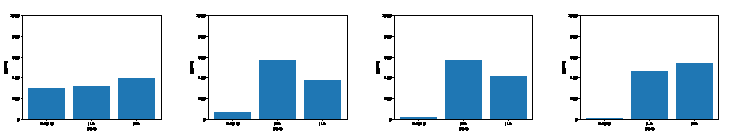
\includegraphics[width=1.5\textwidth]{col_d_0_r_0_rc_0_steps_1_2_4_8.pdf} \\
\midrule
randomized order, trotter steps = 1, 2, 4, 8 \\
\midrule
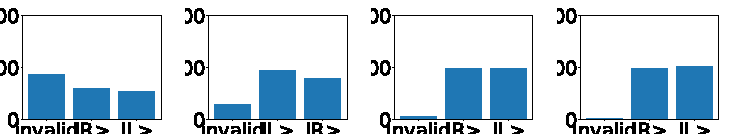
\includegraphics[width=1.5\textwidth]{col_d_0_r_1_rc_0_steps_1_2_4_8.pdf} \\
\bottomrule
\end{tabular}
%\end{table}
\end{document}
